\section{Resultados y evaluación}

\subsection{Comparación de modelos}

La Tabla~\ref{tab:resultados-av4} contiene exclusivamente las nuevas ejecuciones
de este avance. Todos los resultados se calcularon sobre 3,712 imágenes reales
de validación, sin aumentos, y corresponden a un checkpoint identificado. Se
conservan los históricos de entrenamiento y las predicciones por imagen.

\begin{table*}[htbp]
\centering
\caption{Resultados nuevos; el checkpoint de cada modelo se selecciona por F1 macro.}
\label{tab:resultados-av4}
\small
\begin{tabular}{lrrrrrr}
\toprule
Modelo & Parámetros & Época & Exactitud (\%) & F1 macro & Pérdida & Tiempo (s) \\
\midrule
MLP de referencia & 9,660,776 & 77 & 15.52 & 0.0280 & 3.403 & 336.7 \\
CNN original & 480,936 & 53 & 63.25 & 0.5740 & 1.520 & 525.8 \\
CNN + 2 convoluciones & 1,218,600 & 46 & 62.23 & 0.5502 & 1.786 & 500.6 \\
CNN + AdamW + LR & 480,936 & 61 & 64.44 & 0.5745 & 1.507 & 605.6 \\
\bottomrule
\end{tabular}
\par\smallskip
\parbox{0.95\textwidth}{\footnotesize Época: checkpoint seleccionado, no número total
de épocas ejecutadas. Tiempo: entrenamiento, excluyendo evaluación y generación
de figuras. La MLP es una referencia reconstruida; no un resultado histórico
atribuible al Avance 3. Una sola semilla por modelo.}
\end{table*}

\begin{figure*}[htbp]
\centering
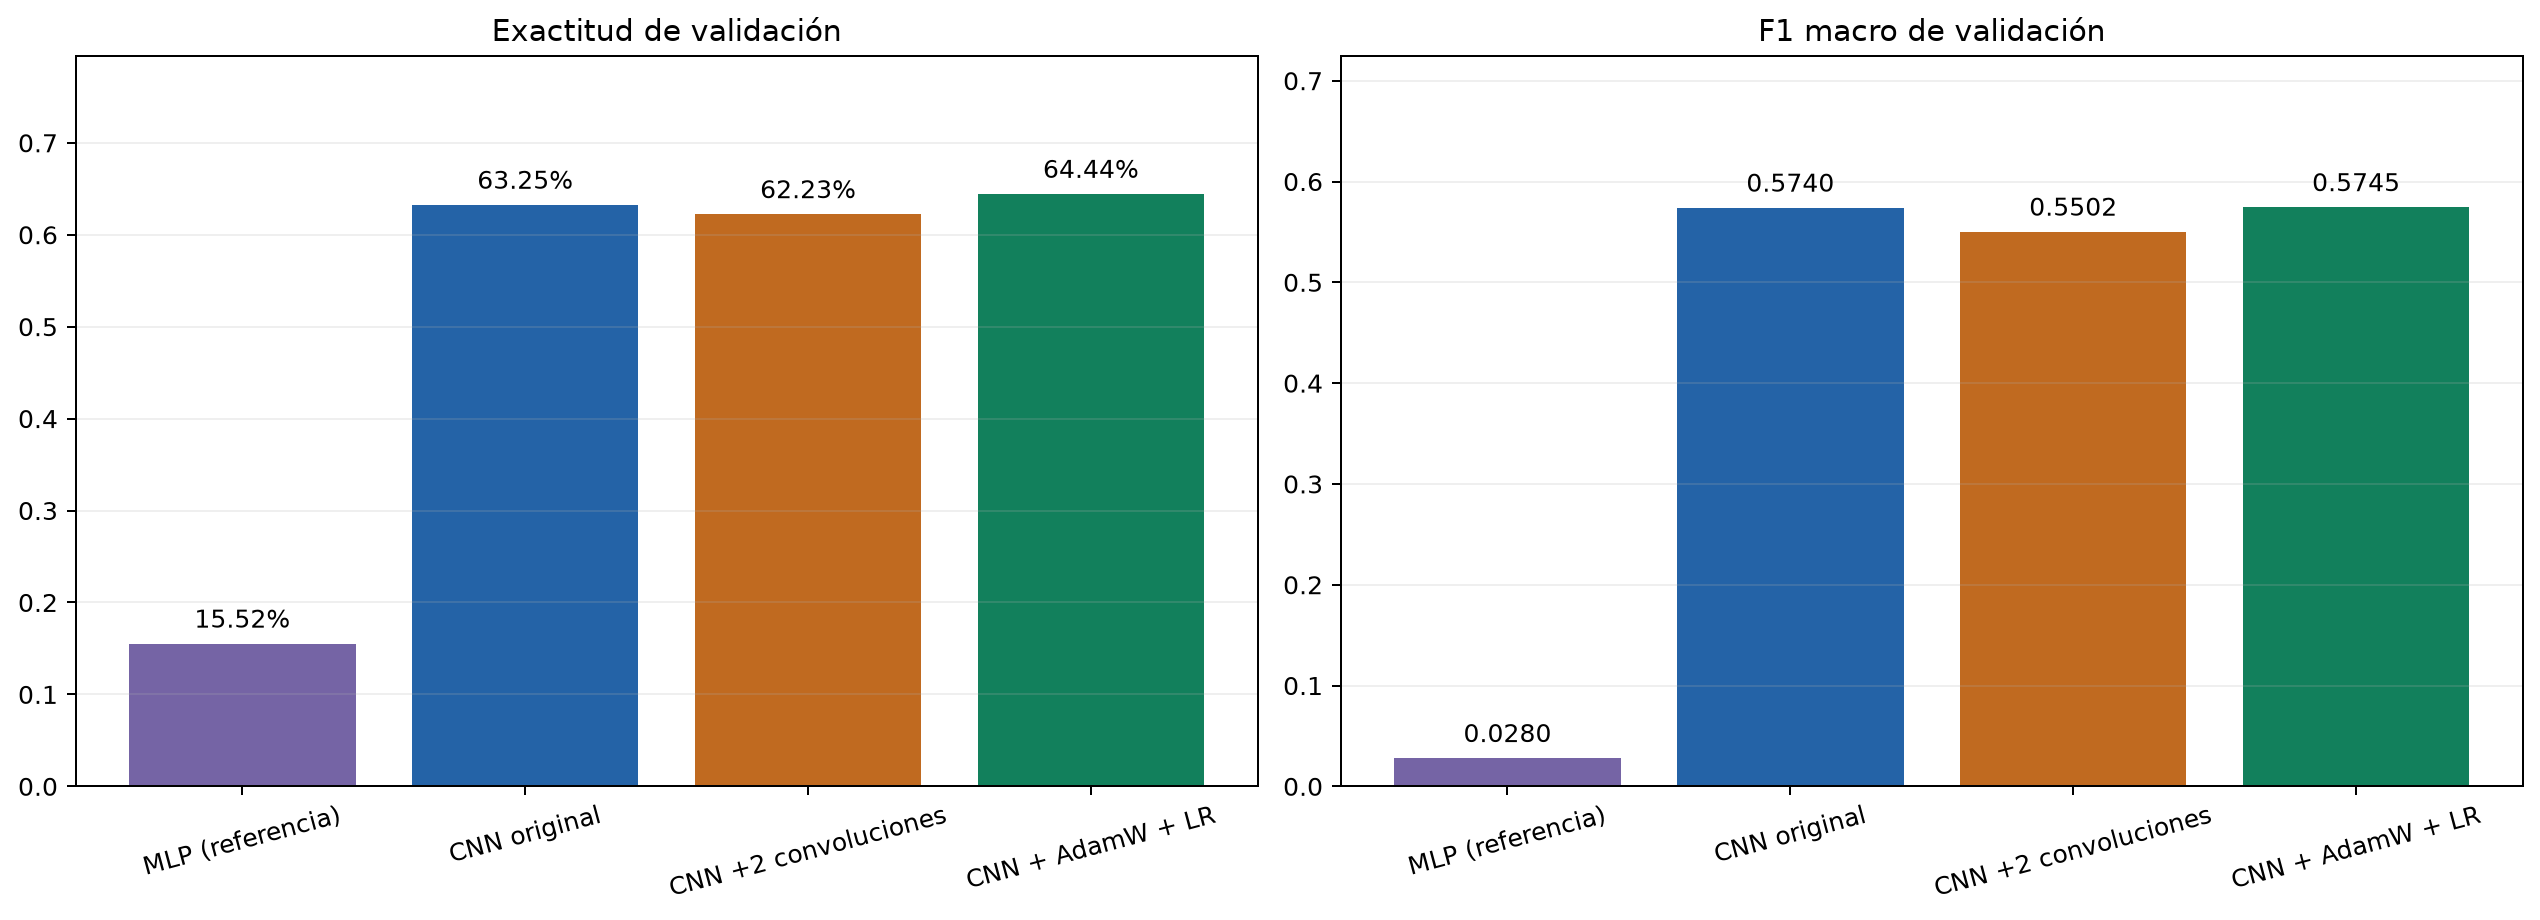
\includegraphics[width=\textwidth]{avance4_2026-10-21/figures/comparacion_metricas.png}
\caption{Exactitud y F1 macro sobre la misma validación. El modelo elegido se
determina por F1 macro y puede diferir del que maximiza la exactitud.}
\label{fig:metricas-av4}
\end{figure*}

\subsection{Puente entre la red totalmente conectada y la CNN}

La CNN original obtuvo 63.25\% de exactitud frente a 15.52\% de la red totalmente conectada de referencia (+47.74 puntos porcentuales). F1 macro cambió de 0.0280 a 0.5740. La MLP tiene 9,660,776 parámetros frente a 480,936 de la CNN.

El resultado es compatible con la ventaja de compartir filtros y preservar vecindarios de píxeles: una CNN puede reutilizar patrones locales sin asignar un peso independiente a cada píxel de cada posición. GAP también limita los parámetros de la etapa densa. Esta explicación es una interpretación arquitectónica del resultado, no una prueba causal aislada; ambas redes tienen distinta capacidad y pueden requerir otros hiperparámetros. Si la MLP presenta baja exactitud tanto en entrenamiento como en validación, su limitación es de ajuste u optimización y no se debe diagnosticar como sobreajuste solo porque rinda peor que la CNN.

La comparación solicitada con el modelo exacto entregado en el Avance 3 queda limitada por la ausencia de ese artefacto identificado. El experimento reconstruido permite comparar familias de modelos en condiciones comunes, sin inventar resultados históricos. El primer intento con Adam a $10^{-3}$ predijo una sola clase (5.82\% de exactitud, F1 macro 0.0011); se conserva como diagnóstico. La referencia final utiliza $10^{-4}$ y mayor paciencia. Esta adaptación de optimización se declara para no atribuir exclusivamente a la arquitectura todas las diferencias observadas.

\subsection{Efecto de agregar dos convoluciones}

La versión de seis convoluciones obtuvo 62.23\% de exactitud y F1 macro 0.5502. Frente a la CNN original, la diferencia es -1.02 puntos de exactitud y -0.0238 de F1 macro. Los parámetros aumentan de 480,936 a 1,218,600. Agregar profundidad incrementa la capacidad de representación, pero no garantiza mejorar validación: también modifica la optimización y puede facilitar el sobreajuste. La conclusión corresponde a esta configuración y semilla, sin afirmar superioridad universal de una profundidad.

\subsection{Modelo elegido y análisis de errores}

Se conserva \textbf{CNN + AdamW + LR}, por tener el mayor F1 macro de esta comparación: 0.5745, con exactitud 64.44\%, pérdida 1.507 y checkpoint en la época 61. La Figura~\ref{fig:confusion-av4} muestra la matriz de confusión normalizada por clase real. La diagonal representa recall por clase; los valores fuera de ella son errores. Se entregan además la matriz de conteos, los CSV de ambas matrices y las predicciones individuales.

\begin{figure*}[p]
\centering
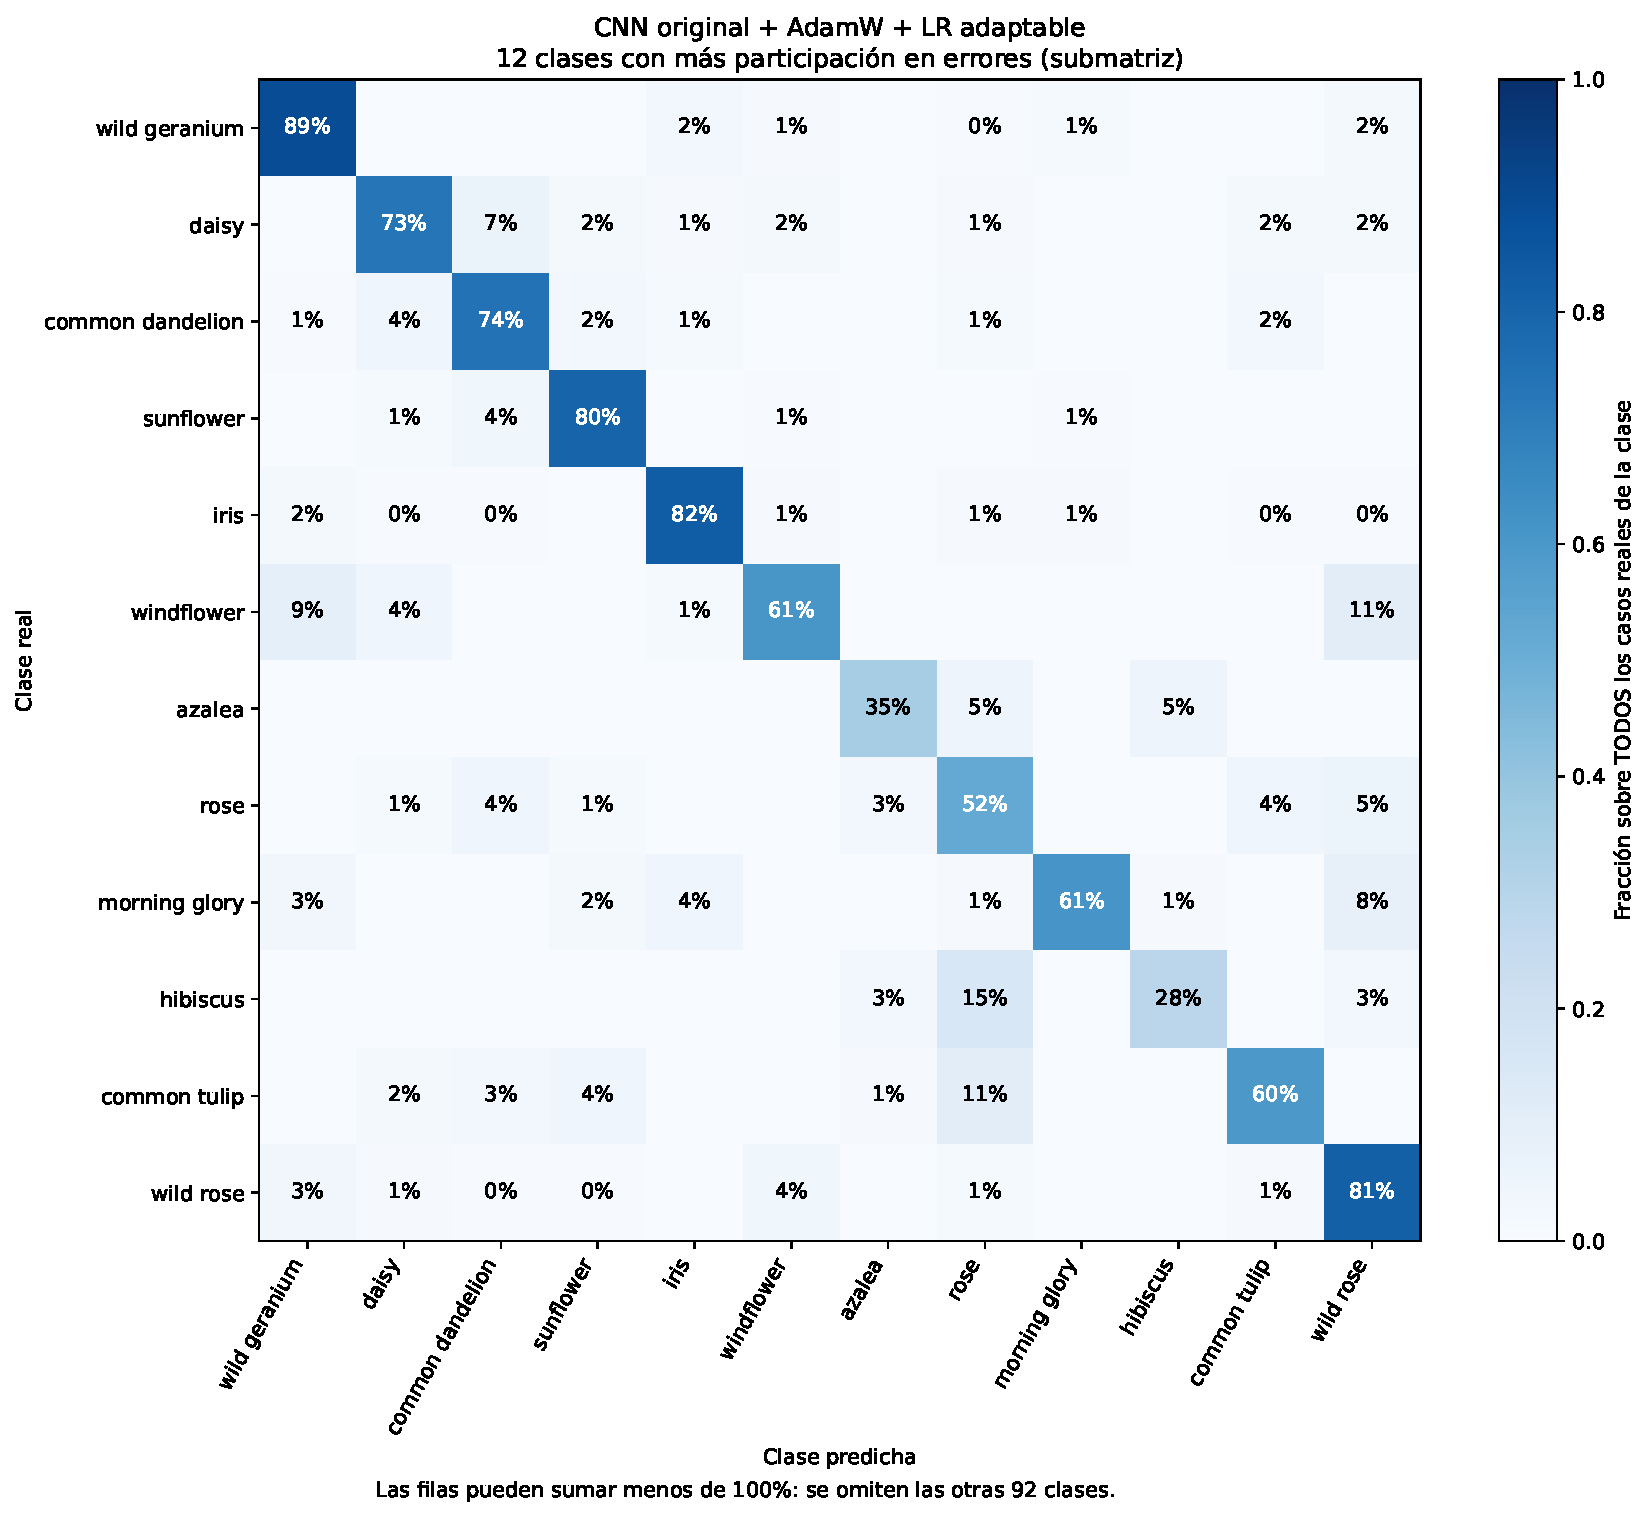
\includegraphics[width=\textwidth]{avance4_2026-10-21/figures/cnn_regularizada/confusiones_principales.pdf}
\caption{Vista legible de las 12 clases con mayor participación en errores. Es una submatriz de la matriz completa: los porcentajes se calculan sobre todos los ejemplos reales de cada clase y las filas mostradas pueden sumar menos de 100\%.}
\label{fig:confusiones-foco-av4}
\end{figure*}

\begin{figure*}[p]
\centering
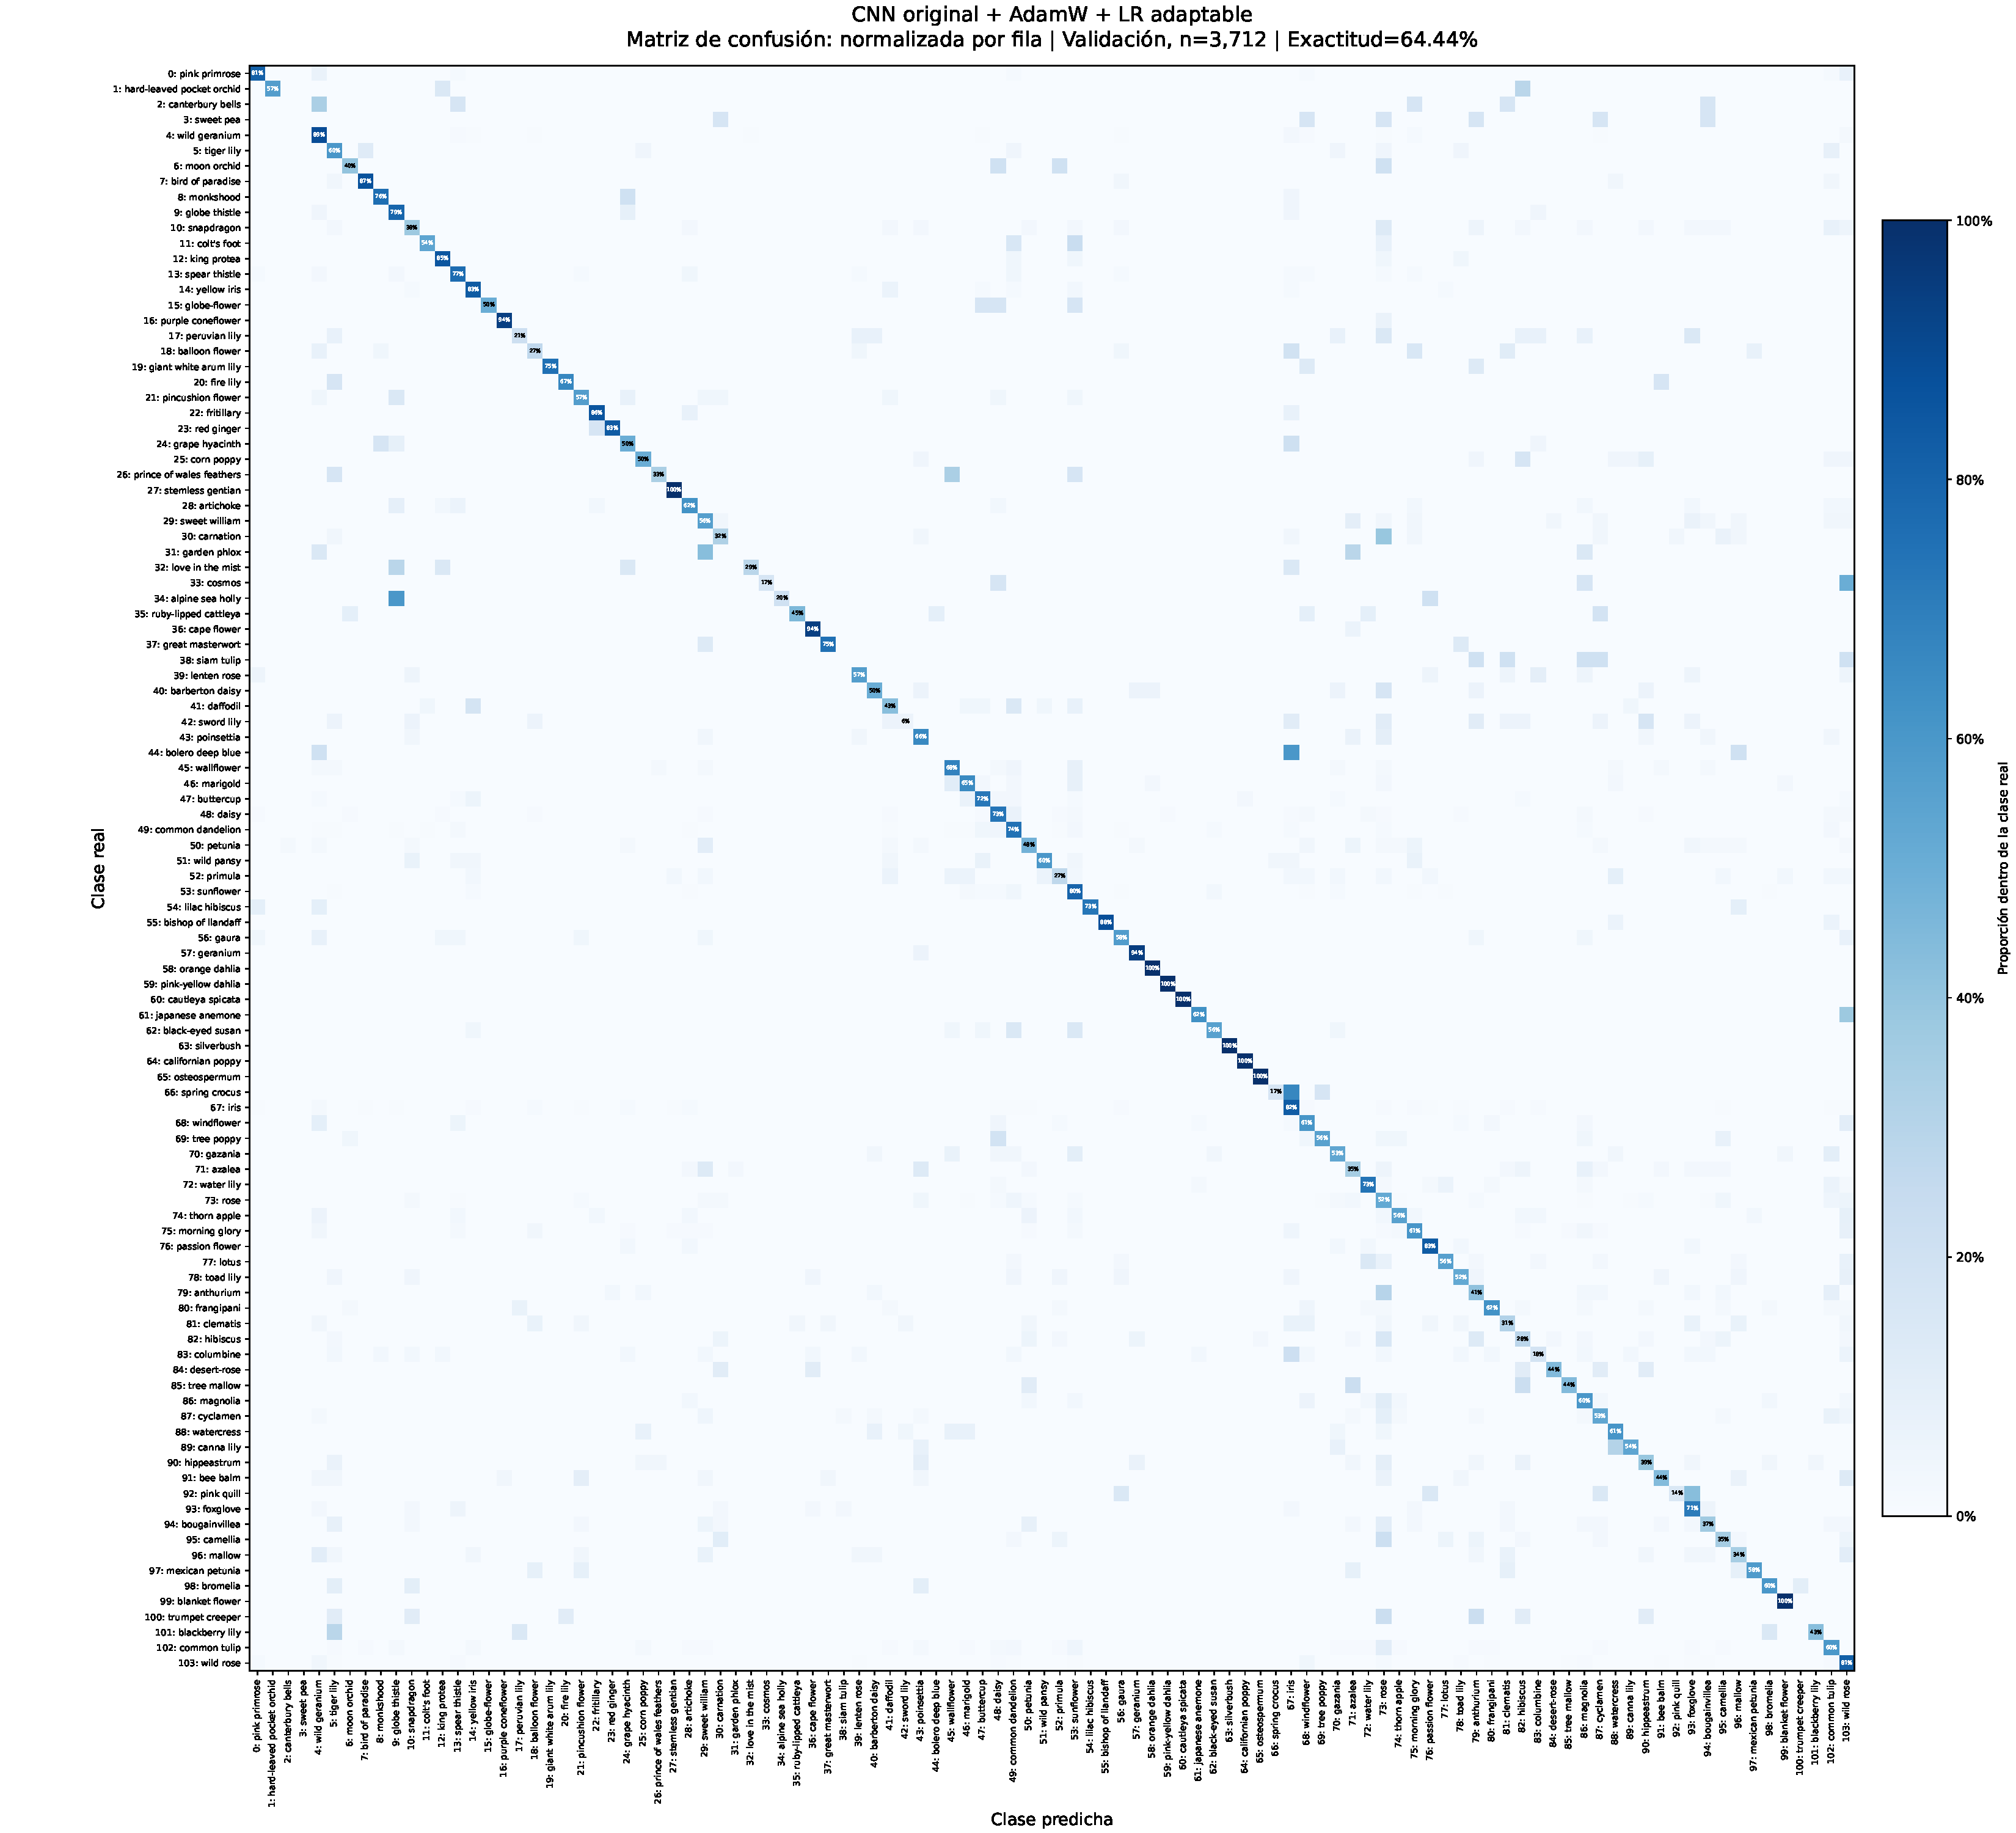
\includegraphics[width=\textwidth,height=0.85\textheight,keepaspectratio]{avance4_2026-10-21/figures/cnn_regularizada/confusion_matrix_normalized.pdf}
\caption{Matriz de confusión del modelo elegido sobre validación. Filas: clase real; columnas: clase predicha. Normalización por fila. Se conserva la versión de alta resolución con las 104 clases.}
\label{fig:confusion-av4}
\end{figure*}

Algunos de los pares más confundidos son:
\begin{itemize}
\item common tulip predicha como rose: 12 imágenes.
\item carnation predicha como rose: 12 imágenes.
\item anthurium predicha como rose: 10 imágenes.
\item windflower predicha como wild rose: 8 imágenes.
\item wild rose predicha como windflower: 8 imágenes.
\end{itemize}
La Figura~\ref{fig:predicciones-av4} ilustra aciertos y errores del checkpoint elegido. Se muestran seis de cada tipo, seleccionados con semilla fija, por lo que esa figura no estima la tasa de error global.

\begin{figure*}[p]
\centering
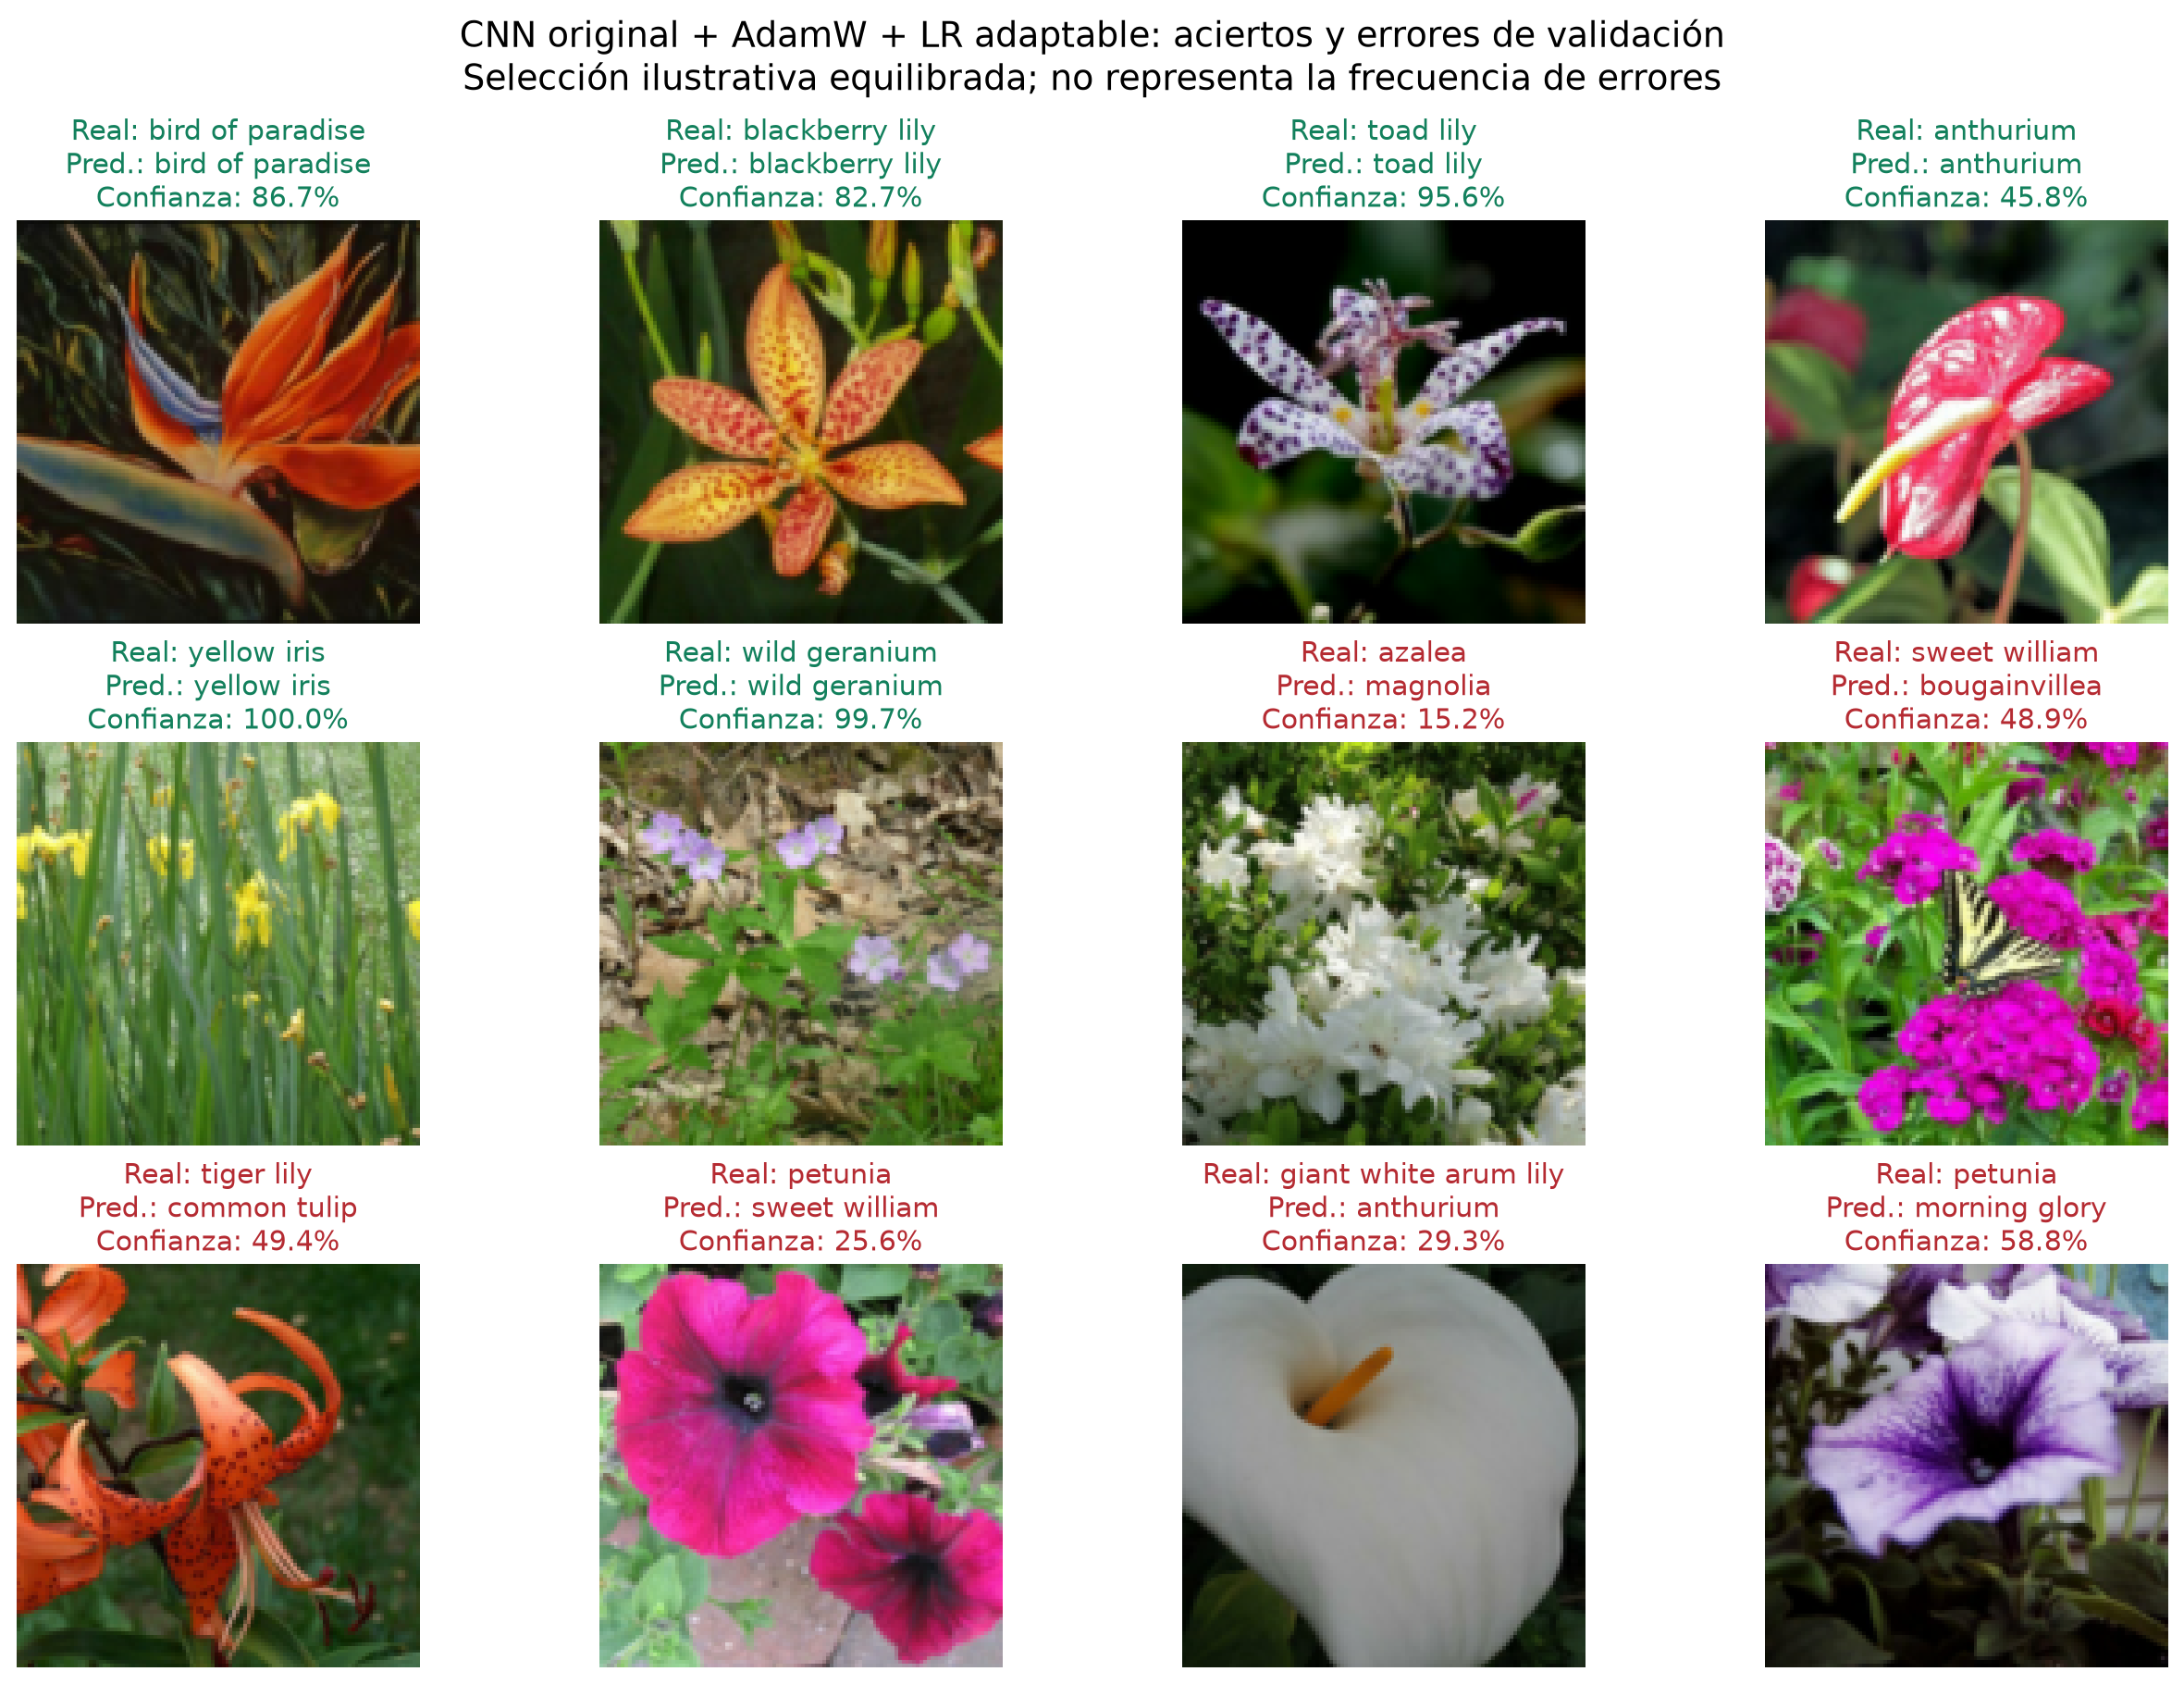
\includegraphics[width=\textwidth]{avance4_2026-10-21/figures/cnn_regularizada/predicciones_ejemplo.png}
\caption{Ejemplos reales de validación con etiqueta verdadera, predicción y confianza softmax. El conjunto mostrado equilibra aciertos y errores solo para facilitar la inspección visual.}
\label{fig:predicciones-av4}
\end{figure*}

\subsection{Conclusiones y limitaciones}

La comparación documenta el cambio de una referencia totalmente conectada a un extractor convolucional, el efecto de aumentar dos convoluciones y el efecto observado de una intervención combinada de regularización. La elección se basa en F1 macro para evitar que las clases numerosas dominen la decisión. Las curvas permiten diagnosticar el comportamiento durante el entrenamiento y justifican conservar checkpoints anteriores al final cuando la validación deja de mejorar.

La validación se utiliza también para selección, los resultados son de una semilla y no se dispone de etiquetas de prueba locales. Harían falta varias semillas, ablaciones controladas y una evaluación independiente para cuantificar incertidumbre y separar el efecto de cada técnica.
